\documentclass[11pt]{article}
\usepackage{import}
\usepackage[margin=1in, top=1in]{geometry}
\usepackage[all]{nowidow}
\usepackage[hyperfigures=true, hidelinks, pdfhighlight=/N]{hyperref}
\usepackage[separate-uncertainty=true, group-digits=false]{siunitx}
\usepackage{graphicx,amsmath,physics,tabto,float,amssymb,pgfplots,verbatim,tcolorbox}
\usepackage{listings,xcolor,subfig,caption,import,wrapfig,lipsum,tikz,biblatex}
\usepackage[version=4]{mhchem}
\usepackage[noabbrev]{cleveref}
\newcommand{\creflastconjunction}{, and\nobreakspace}
\newcommand{\mb}[1]{\mathbf{#1}}
\numberwithin{equation}{section}
\numberwithin{figure}{section}
\numberwithin{table}{section}
\definecolor{stringcolor}{HTML}{C792EA}
\definecolor{codeblue}{HTML}{2162DB}
\definecolor{commentcolor}{HTML}{4A6E46}
\captionsetup{font=small, belowskip=0pt}
\lstdefinestyle{appendix}{
    basicstyle=\ttfamily\footnotesize,commentstyle=\color{commentcolor},keywordstyle=\color{codeblue},
    stringstyle=\color{stringcolor},showstringspaces=false,numbers=left,upquote=true,captionpos=t,
    abovecaptionskip=12pt,belowcaptionskip=12pt,language=Python,breaklines=true,frame=single}
\lstdefinestyle{inline}{
    basicstyle=\ttfamily\footnotesize,commentstyle=\color{commentcolor},keywordstyle=\color{codeblue},
    stringstyle=\color{stringcolor},showstringspaces=false,numbers=left,upquote=true,frame=tb,
    captionpos=b,language=Python}
\renewcommand{\lstlistingname}{Appendix}
\pgfplotsset{compat=1.17}
\addbibresource{bibliography.bib}

\title{{\Huge A ``look-see'' at }}
\author{{\Large Miles Kidson}\\ \\
Supervisors: Prof. Zinhle Buthelezi, Dr. SV Fortsch, \& Prof. Tom Dietel\\
Assisted By: Dr. B Naik (Postdoctoral fellow)}
\date{\textbf{UCT Honours 2022}}

\begin{document}
    
\maketitle

\begin{figure}[h]
    \begin{center}
        
\includegraphics{Figs/UCT.jpg}
    \end{center}
\end{figure}

\begin{abstract}
    \centering
    We investigate preliminary data from proton-proton collisions in Run 3 at ALICE to compare the new Muon Forward Tracker (MFT) to the newly upgraded Inner Tracking System (ITS).
\end{abstract}

\newpage
\tableofcontents

\newpage
\section{Introduction}\label{sec:Introduction}
The Muon Forward Tracker (MFT) is a new detector added to ALICE at CERN for Run 3. Its primary use is to add vertexing capabilities to the Muon Spectrometer (MCH) in the forward region of ALICE. With Run 3 comes a new analysis framework, called Online-Offline (O2), which is better suited to the new ways in which data will be taken for Run 3 due to the increased energy and luminosity. This report aims to use O2 to have a ``look-see'' at data coming from the MFT to see if the detector and analysis tools are working correctly. The data used in this investigation is from two proton-proton collision runs performed in October 2021, at a centre-of-mass energy of \SI{900}{\giga\electronvolt}. This is not an energy we expect to use for physics data analysis---Run 3 is designed to reach $\sqrt{s}=\SI{13.6}{\tera\electronvolt}$---but is good enough for this purpose.

\section{Background}\label{sec:Background}
\subsection{The ALICE Detector}
\begin{itemize}
    \item What is the LHC?
    \item What is ALICE?
    \item What does ALICE look for?
    \item What is Run 3?
\end{itemize}
The ALICE detector (A Large Ion Collider Experiment) is a detector experiment at the Large Hadron Collider (LHC) at CERN. Its primary goal is the investigation of ``strongly interacting matter at extreme energy densities, where a formation of a new phase of matter, the quark-gluon plasma, is expected'' (\cite{ALICE_LOI}). It achieves this goal by studying the products of head-on collisions of heavy ions such as lead. 

% ALICE is situated at 

% The LHC at CERN in Geneva is built to accelerate particles up to very high energies (\SI{13.6}{\tera\electronvolt})

The coordinate system used at ALICE needs to be discussed first in order to fully explain the scope of this report. A modified cylindrical coordinate system is used as most detectors in the experiment are cylindrically symmetric about the beamline of the LHC. We place the $z$-axis along the beamline and call the angle around the $z$-axis $\varphi$, the azimuthal angle. The angle from the $z$-axis to the $x-y$ plane is called $\theta$, the polar angle. 
We are interested in the momentum of particles that we track in the detector, which we call $\vec{p}$, but we also define the transverse momentum $p_{\mathrm{T}}=\sqrt{p_x^2 + p_y^2}$. The last important coordinate to discuss is the rapidity, often denoted as $y$. This is defined as 
\begin{equation}
    y=\frac 12 \ln\left(\frac{E+p_z}{E-p_z}\right)
    \label{eqn:rapidity}
\end{equation}
where $E$ is the total energy of the particle being considered

\begin{figure}[h]
    \begin{center}
        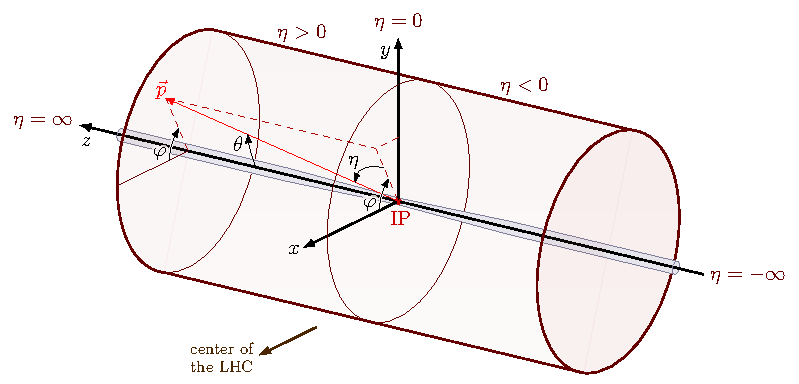
\includegraphics[width=.8\textwidth]{Figs/coords.pdf}
        \caption{Coordinate system \cite{coords}}
        \label{fig:coords}
    \end{center}
\end{figure}


\subsection{Run 3 Specifics}
\begin{itemize}
    \item What was upgraded/added in Run 3?
    \item 
\end{itemize}

\subsection{Muon Forward Tracker}


\printbibliography

\end{document}


